The aim of the superclustering procedure is to collect the majority of
the pixels belonging to a track which is longer and possibly with a pattern
more irregular than the one clustered by \idbscan. The main limitation
of  \idbscan to follow a long track is mainly originated by the irregular behavior of the energy
deposition along the path length.  As can be clearly seen in
Fig.~\ref{fig:basic_clusters} (right), or even in the example of a raw
image of an event with two long cosmic rays in
Fig.~\ref{fig:typicalimage1} (right), clusters with larger energy
release are followed by regions along the path with a lower or even a
zero release.  These local minima are sometimes as large, in the 2D
space, as the typical size of the $\epsilon$ parameter of
\dbscan~\cite{dbscan}. Despite the low electronic noise of the
ORCA-Flash 4.0 camera sensor, the energy releases in these local
minima are similar in magnitude to the average single-pixel noise.
The \idbscan is limited in connecting the full length of an extended
path, because of two reasons. First, inflating $\epsilon$ parameter as
much as needed to cover the areas of local minima conflicts with the
need to reject noise around the cluster.  The \idbscan parameters are
optimized for the \lemon running conditions to collect most of the
signals of $E \approx 5$\keV and rejecting the typical noise of
$\approx 1$ photon per pixel. This avoids collecting extra noise in
the cluster, biasing the energy scale and worsening its resolution,
and keeps the rate of fake clusters at a negligible level.  This is
studied in great detail in Ref.~\cite{iDBSCAN}.  Second, the iterative
nature of the algorithm with very different parameters for each
iteration, each tuned for very different intensity, makes it
convenient and efficient for a deposition of a fixed energy density
(like the spots originating from the \fe source), but not for the cases
like the Fig.~\ref{fig:basic_clusters} (right), where the same track
is split in several parts, with some of them in different iterations.
This requires a method that can continuously follow the pattern of the
track, profiting of the full resolution image, where the {\it gradients} of
the energy deposition along the track trajectory are smaller than the
ones in the transverse direction. Running any of the most common
methods on the full $1024\times1024$ image is not manageable CPU-wise,
due to huge combinatorics while maintaining the limited zero-suppression
described previously.

The procedure adopted for the final supercluster reconstruction in the
\lemon detector starts from defining the \textit{interesting regions}
in the image that may contain pixels from an energy deposit. These are
identified by the basic cluster algorithm \idbscan previously
described and run  \textcolor{red}{run ??} in the $512\times512$ reduced-resolution image. In
order to gather the peripheral pixels, especially along the track
trajectory where breaks in sub-basic clusters may have happened, a
window of $5\times5$ pixels is considered, around each pixel belonging
to a macro-pixel clustered in a basic cluster. A full resolution image
formed only by the interesting pixels passing the simple initial
filtering described in Sec.~\ref{sec:zerosuppression} is formed.  The
gradients of such image are computed pixel-by-pixels to look for the
edge region where the image changes from signal to noise-only:
\begin{equation}
\label{eq:gradient}
\vert\vert\nabla(N)\vert\vert =
\sqrt{\left(\frac{\partial N}{\partial x}\right)^2
  +\left(\frac{\partial N}{\partial y}\right)^2},
\end{equation}
and the gradient direction is given by:
\begin{equation}
  \label{eq:graddir}
  \theta = \tan^{-1}\left(\frac{\partial N}{\partial y}/\frac{\partial N}{\partial x}\right).
\end{equation}
In order to reduce the effect of the noise which makes the first
derivatives in Eq.~\ref{eq:gradient} to fluctuate, a Gaussian
filtering is applied, with a 5$\sigma$ threshold, where $\sigma$ is
the standard deviation of the intensities of the pixels considered.

After this filtering is applied, the superclustering algorithm is an
application of the \textit{morphological geodesic active
  contours}\cite{gac,mgac}, called \gac in the following.  This method
us an active contour finding algorithm, widely used in computer
vision, where the boundary curve $\mathcal{C}$ of an object is
detected by minimizing the \textit{energy} associated to $\mathcal{C}$:
\begin{equation}
  \label{eq:gacenergy}
  E(\mathcal{C}) = \int_{0}^{1} g(N)(\mathcal{C}(p)) \cdot \vert\mathcal{C}_p\vert dp,
\end{equation}
where $N$ is the number of photons in the pixel (intensity), $ds=
\vert\mathcal{C}_p\vert dp$ is the arc-length parametrization of the
curve in the 2D space, and $g$ is the stopping edge function, which
allows to select the boundary of the cluster.  In the \gac method used
here, the $g$ function is purely geometrical, and uses geodesics of
the image, \ie, local minimal distance path between points with the
same gradient, defined before. The function $g(N)$ is given by:
\begin{equation}
g(N) = \frac{1}{\sqrt{1+\alpha\vert\nabla G_\sigma * N\vert}},
\end{equation}
which is minimal in the edges of the image.  The
$G_\sigma * N$ is the aforementioned Gaussian filter with standard
deviation $\sigma=5$, and the parameter $\alpha$, which regulates the
strength of the filtering is tuned on typical \lemon images to be
$\alpha=100$.

This method has been chosen because it allows to follow track patterns
that may vary from convex to concave shape, and also have kinks, in
cases of $\delta$-rays. To improve the shrinking of the cluster
boundary in the cases of concave-convex tracks, the \textit{balloon}
force~\cite{mgac} is set to -1, in order to push the contour towards a
border in the areas where the gradient is too small. A number of 300
iterations is used to evolve the supercluster contour.

The supercluster obtained on the same track shown in
Fig.~\ref{fig:basic_clusters} (right) after the basic clustering step,
is shown again in full resolution, zoomed around the cluster, in
Fig.~\ref{fig:super_clusters1} (left). The output of the
superclustering with the \gac algorithm is shown on the rihgt panel of
the same figure. The splitting of the clustering present after the
basic cluster step has been recovered, and sections with high density
and low density along the path of the energy deposition have been
joined. Other three examples of superclustered images are shown in
Fig.~\ref{fig:super_clusters2}, in runs without any radioactive
source. The top left panel shows an example of a cosmic ray track
fully reconstructed by the \gac superclustering, which also includes a
$\delta$-ray in the middle of the track length. The top right panel shows an
example of curly track from a candidate of natural radioactivity
interaction; bottom panel shows an example where both a cosmic ray and
a curly track are present. In this case, the extremes of the long and
straight track are still split, but this is much rarer than with the
basic clustering, and it happens when the local minimal along the
trajectories are compatible with noise-only for more than
$\approx$1\unit{cm}.
%
\begin{figure}[ht]
  \begin{center}
     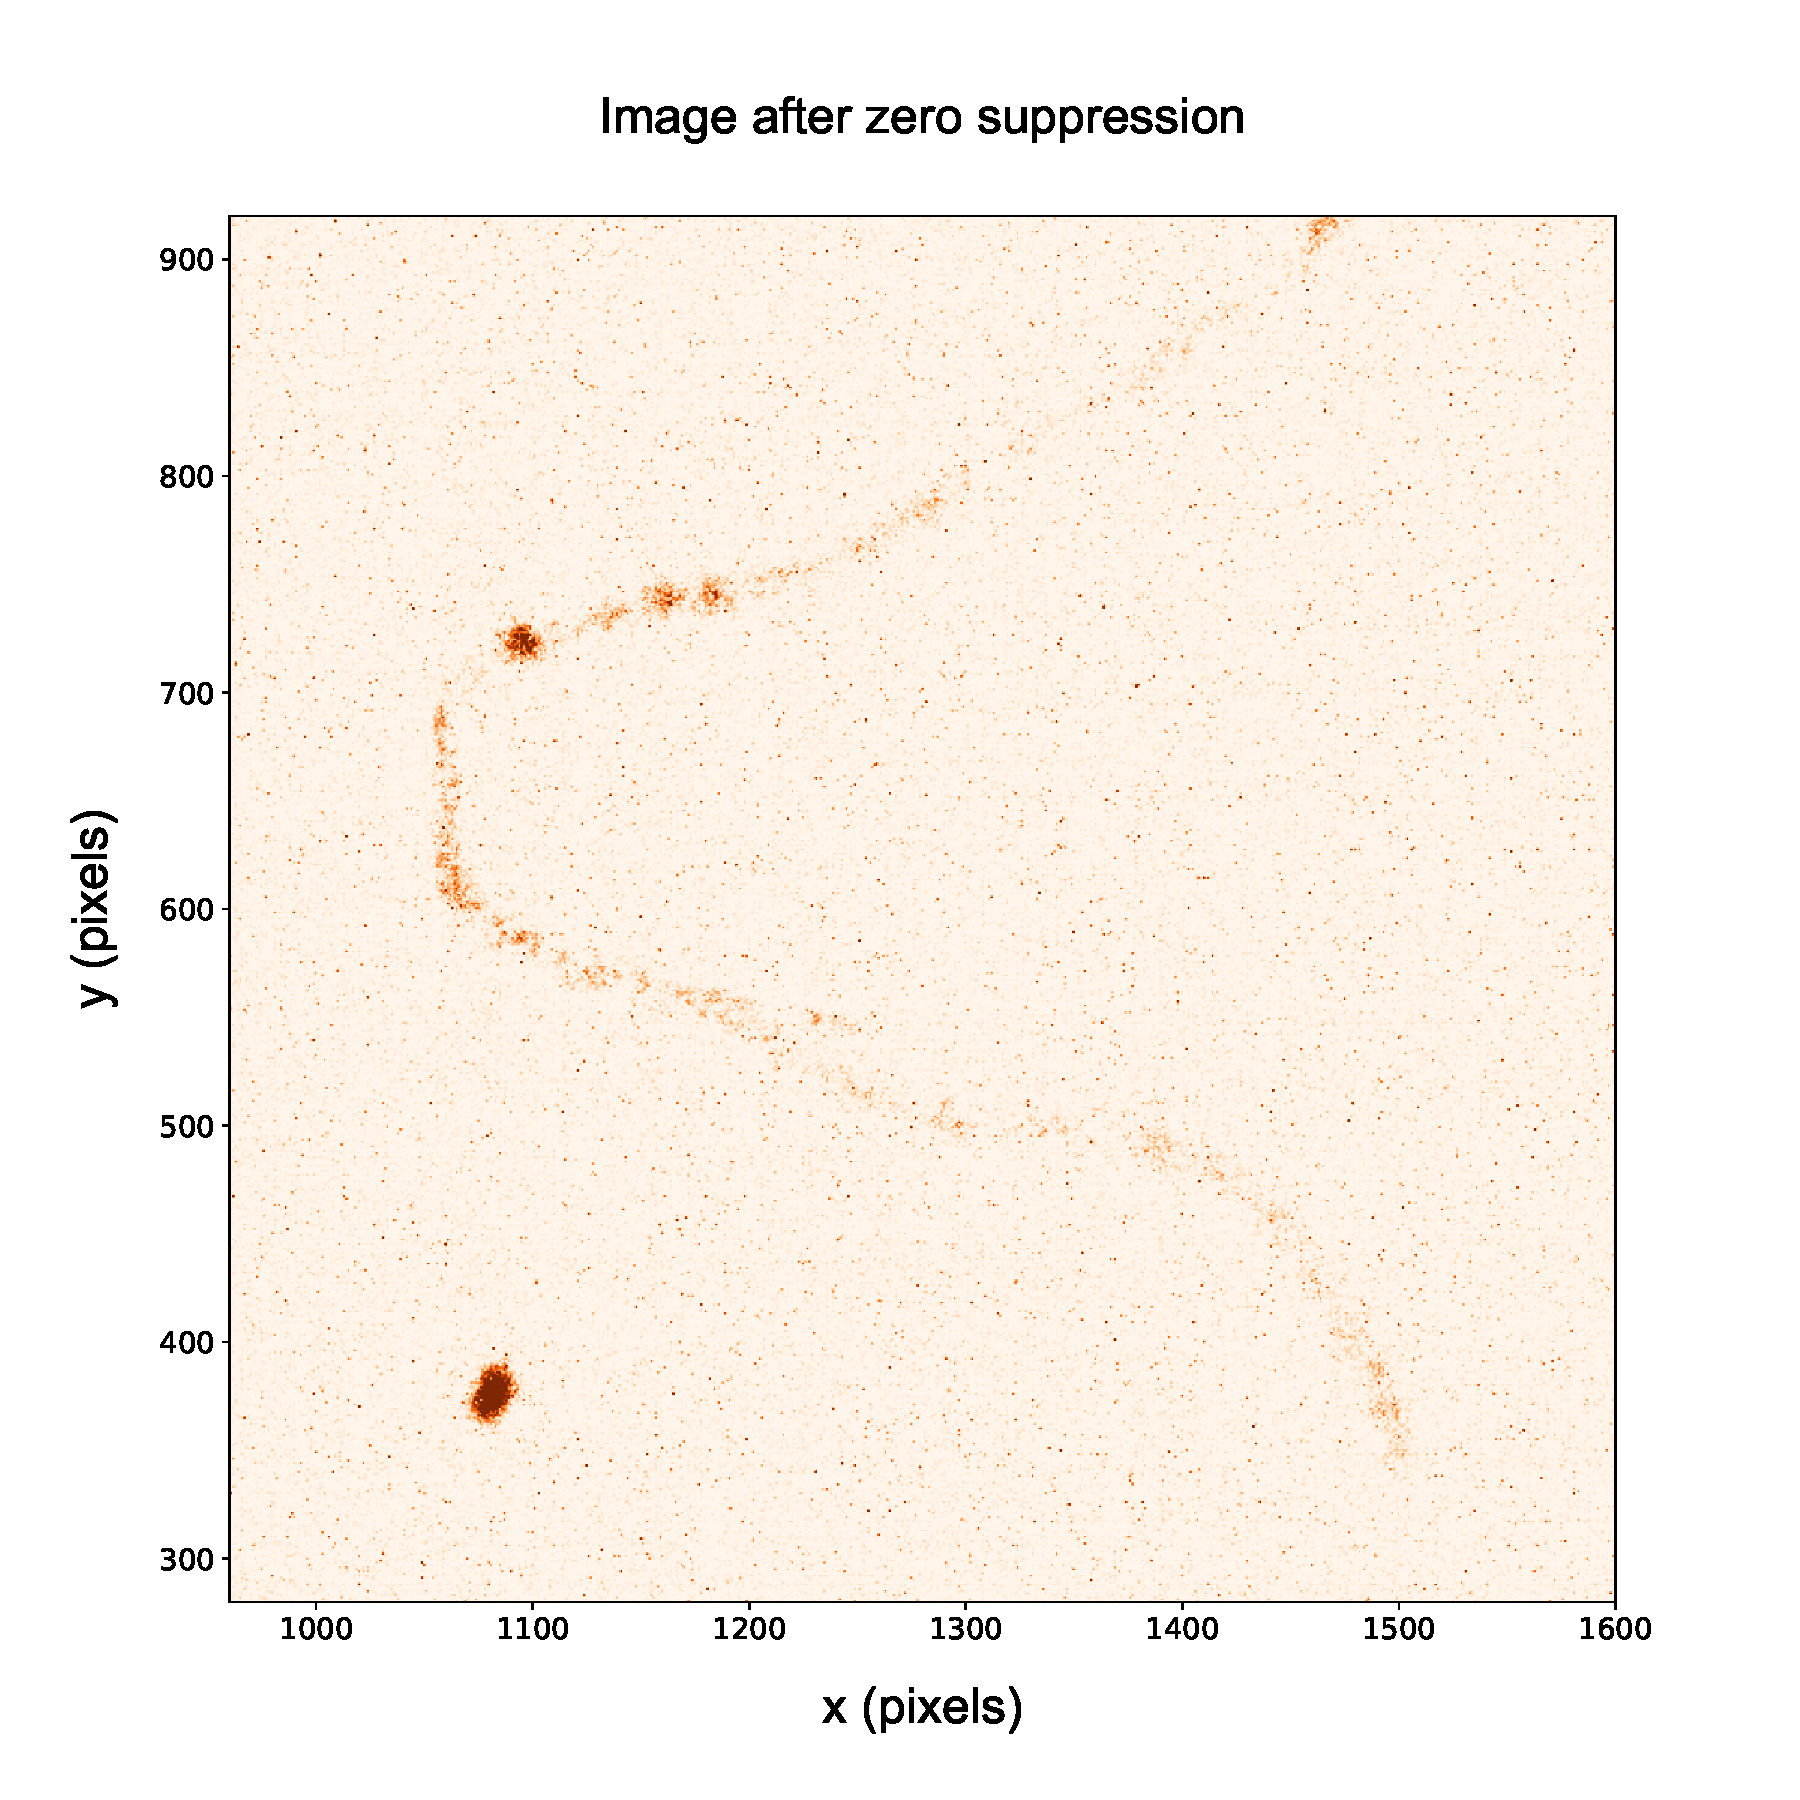
\includegraphics[width=0.49\linewidth]{figures/pic_run02317_ev8_oriIma_paper_zoom}
      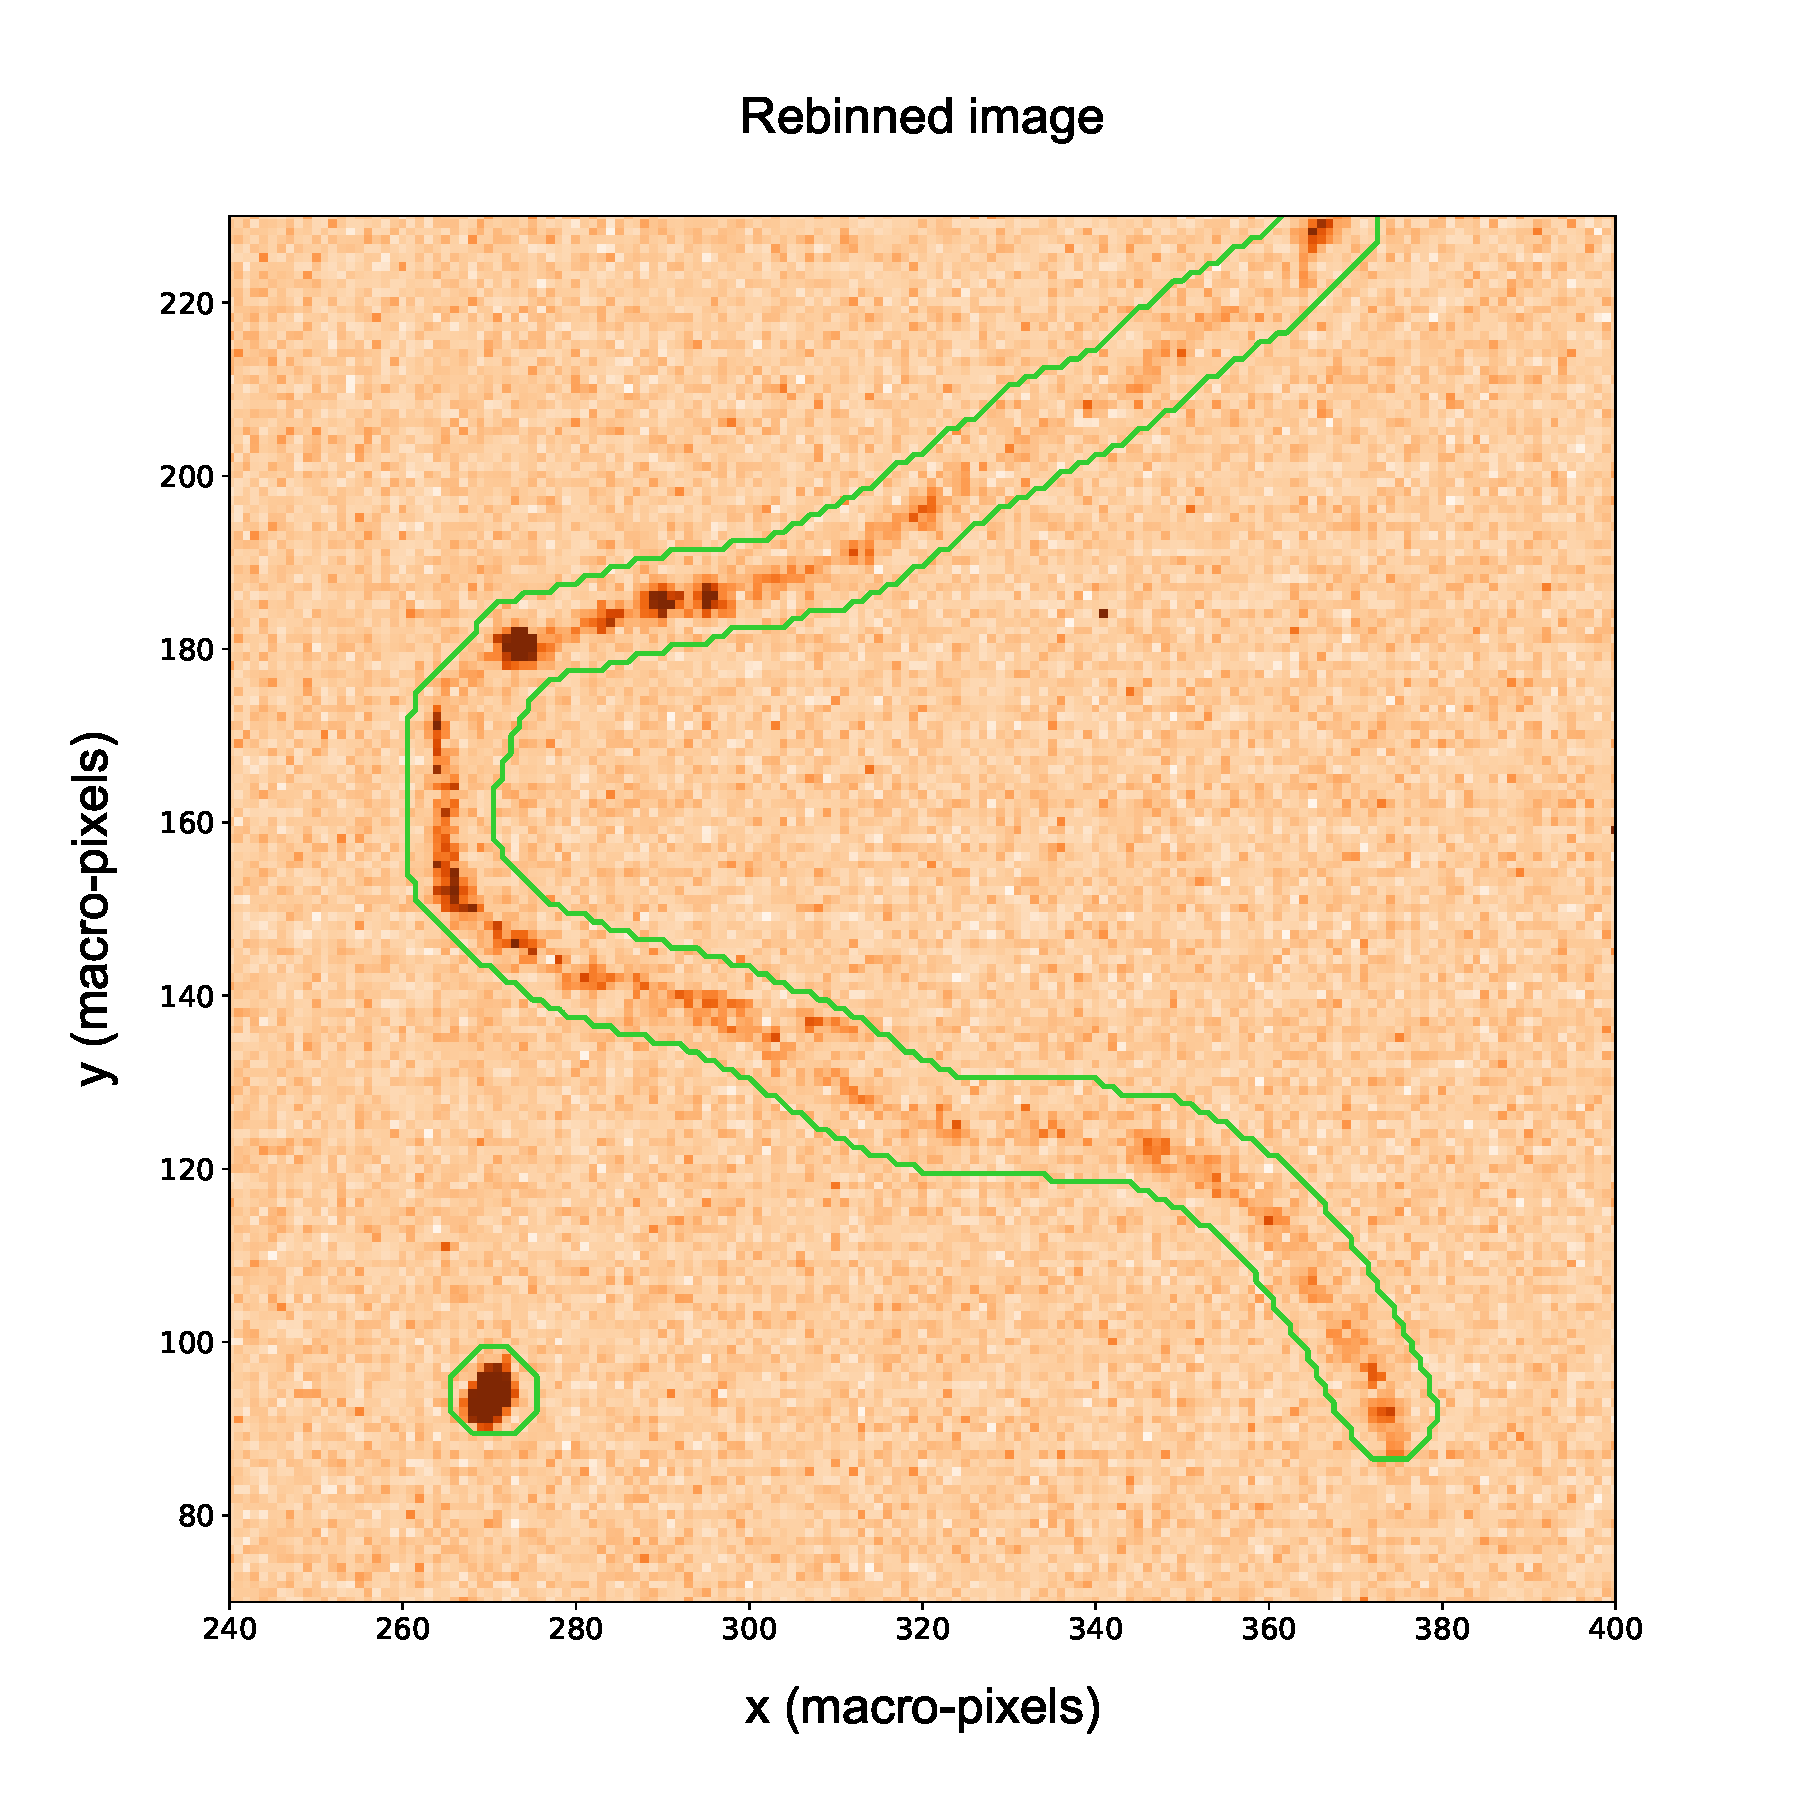
\includegraphics[width=0.49\linewidth]{figures/pic_run02317_ev8_sc_3D_paper}
      \caption{Left: zoom on the full-resolution image of a
        track candidate in a run with \ambe radioactive
        source. Right: output of the superclustering on the rebinned
        image. \label{fig:super_clusters1}}
  \end{center}
\end{figure}
%
\begin{figure}[ht]
  \begin{center}
     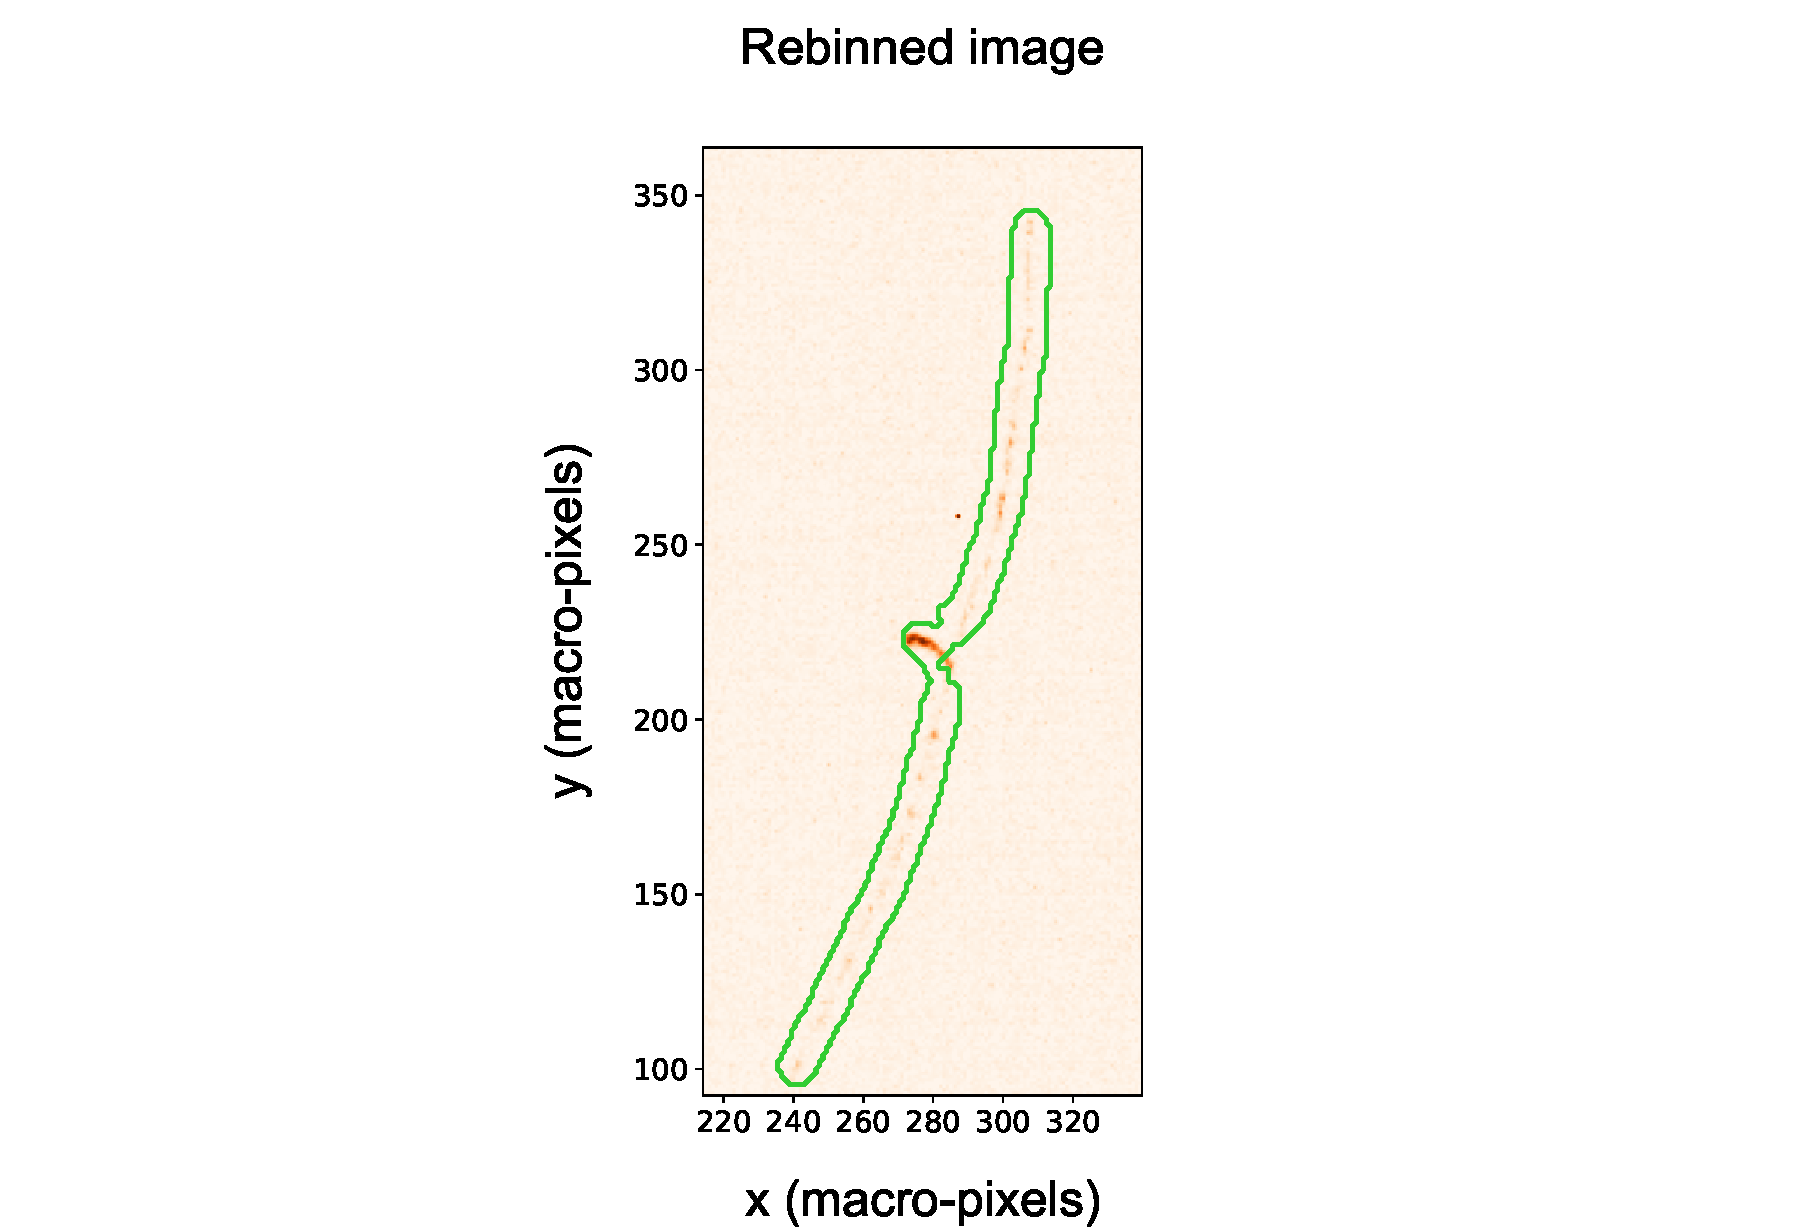
\includegraphics[width=0.49\linewidth]{figures/pic_run02156_ev49_sc_3D_paper}
     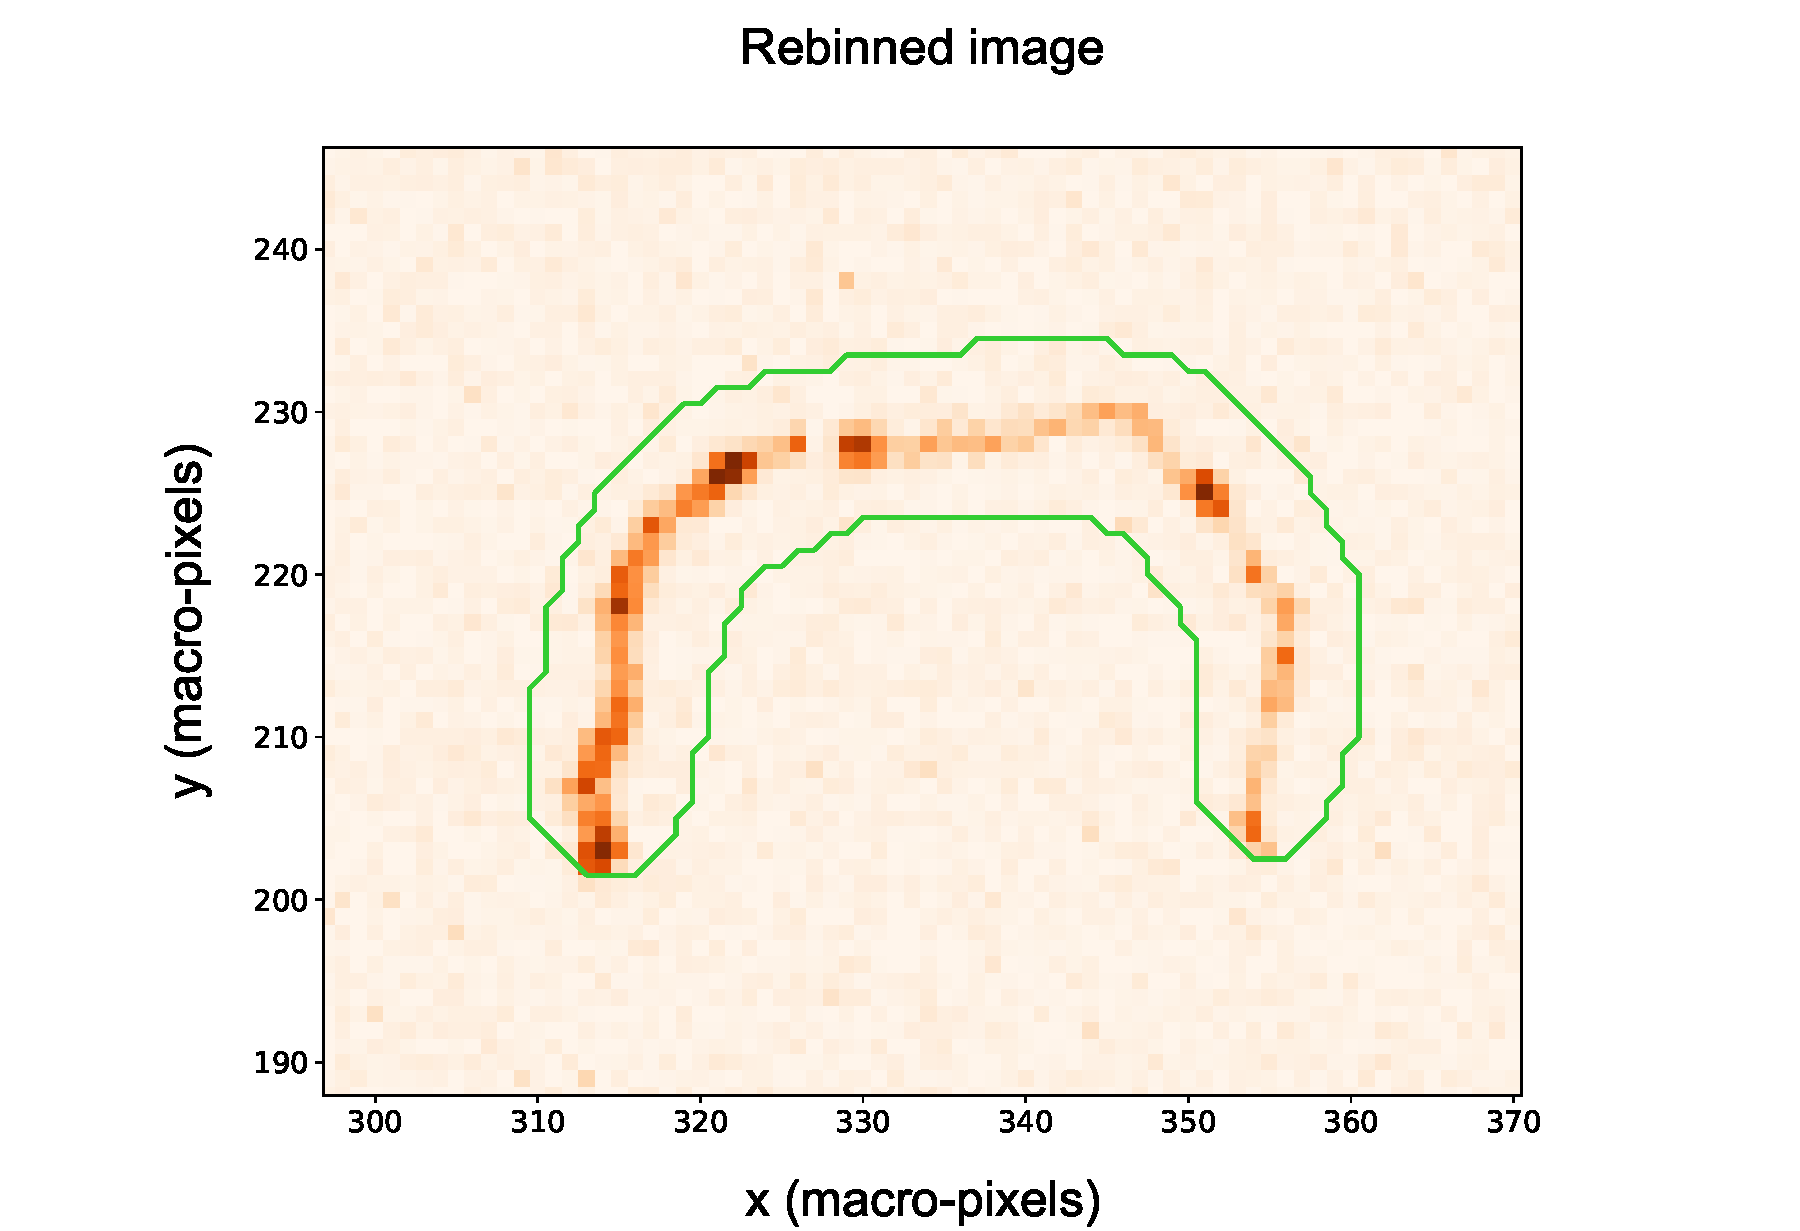
\includegraphics[width=0.49\linewidth]{figures/pic_run02156_ev641_sc_3D_paper} \\
     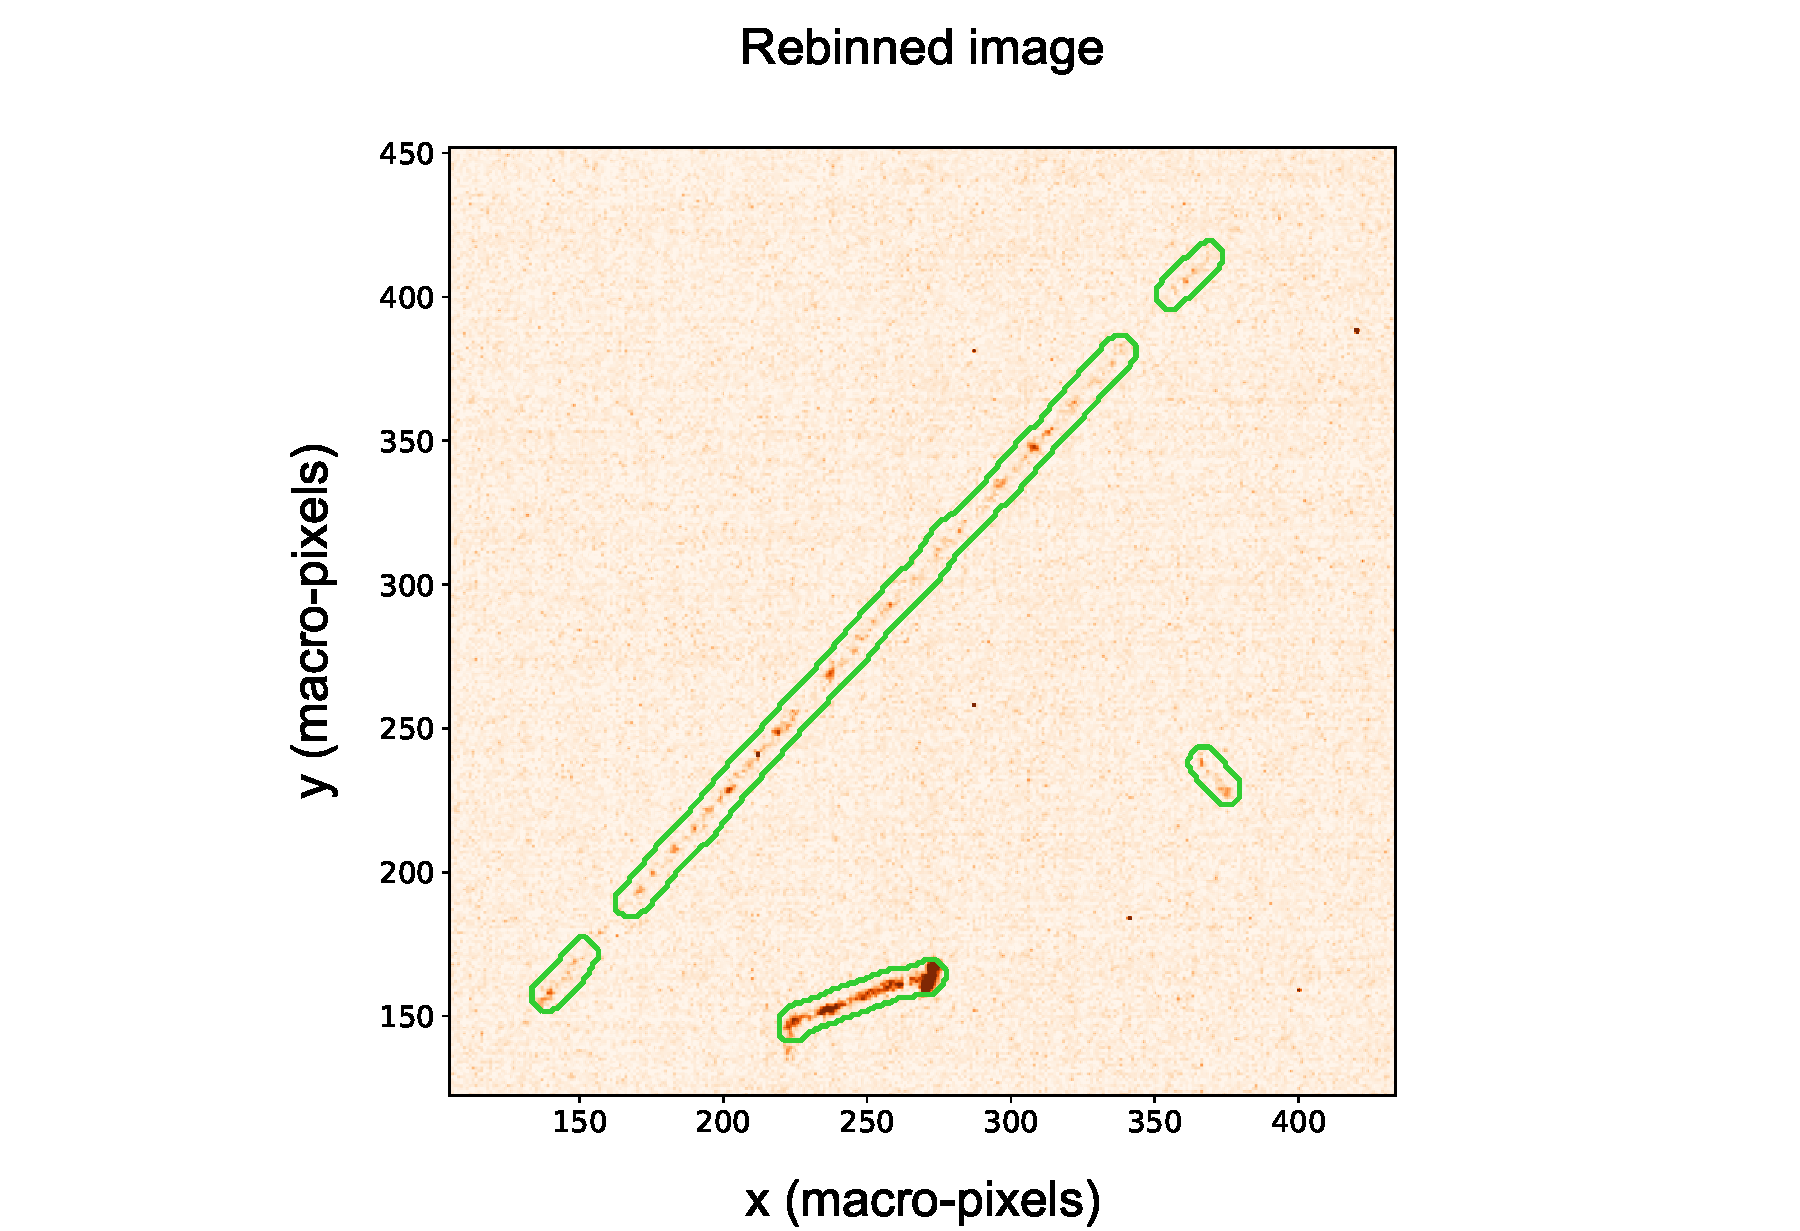
\includegraphics[width=0.6\linewidth]{figures/pic_run02156_ev631_sc_3D_paper}
     \caption{Superclusters reconstructed in a run without radioactive
       sources.  Top left: cosmic ray track fully reconstructed by the \gac
       superclustering. A $\delta$-ray is included in the supercluster. Top right: curly track from a candidate of
       natural radioactivity interaction. Bottom: a cosmic ray with the
       extremes not joined to the main track, plus a curly track from
       natural radioactivity. \label{fig:super_clusters2}}
  \end{center}
\end{figure}
